\documentclass[tikz,border=8pt]{standalone}
% Shared look for every TikZ diagram. Load with % Shared look for every TikZ diagram. Load with % Shared look for every TikZ diagram. Load with \input{../../tools/tikz-style.tex}
\usepackage[T1]{fontenc}
\usepackage{lmodern}
\renewcommand{\sfdefault}{lmr}  % diagrams use the same serif as the text
\usetikzlibrary{arrows.meta, positioning, shapes.geometric, calc, fit, backgrounds}
\definecolor{cblue}{HTML}{4C78A8}
\definecolor{corange}{HTML}{F58518}
\definecolor{cgreen}{HTML}{54A24B}
\definecolor{cred}{HTML}{E45756}
\definecolor{cpurple}{HTML}{B279A2}
\definecolor{cgrey}{HTML}{6B6B6B}
\tikzset{
  every picture/.style={font=\sffamily, line width=1.2pt},
  box/.style={draw=#1, fill=#1!12, rounded corners=4pt, align=center, inner sep=7pt, minimum height=1.1cm},
  box/.default=cgrey,
  arrow/.style={-{Stealth[length=3mm]}, draw=cgrey, line width=1.4pt},
  title/.style={font=\sffamily\bfseries\Large},
  note/.style={font=\sffamily\small, text=cgrey, align=center},
}
\AtBeginDocument{\hyphenpenalty=10000 \exhyphenpenalty=10000}

\usepackage[T1]{fontenc}
\usepackage{lmodern}
\renewcommand{\sfdefault}{lmr}  % diagrams use the same serif as the text
\usetikzlibrary{arrows.meta, positioning, shapes.geometric, calc, fit, backgrounds}
\definecolor{cblue}{HTML}{4C78A8}
\definecolor{corange}{HTML}{F58518}
\definecolor{cgreen}{HTML}{54A24B}
\definecolor{cred}{HTML}{E45756}
\definecolor{cpurple}{HTML}{B279A2}
\definecolor{cgrey}{HTML}{6B6B6B}
\tikzset{
  every picture/.style={font=\sffamily, line width=1.2pt},
  box/.style={draw=#1, fill=#1!12, rounded corners=4pt, align=center, inner sep=7pt, minimum height=1.1cm},
  box/.default=cgrey,
  arrow/.style={-{Stealth[length=3mm]}, draw=cgrey, line width=1.4pt},
  title/.style={font=\sffamily\bfseries\Large},
  note/.style={font=\sffamily\small, text=cgrey, align=center},
}
\AtBeginDocument{\hyphenpenalty=10000 \exhyphenpenalty=10000}

\usepackage[T1]{fontenc}
\usepackage{lmodern}
\renewcommand{\sfdefault}{lmr}  % diagrams use the same serif as the text
\usetikzlibrary{arrows.meta, positioning, shapes.geometric, calc, fit, backgrounds}
\definecolor{cblue}{HTML}{4C78A8}
\definecolor{corange}{HTML}{F58518}
\definecolor{cgreen}{HTML}{54A24B}
\definecolor{cred}{HTML}{E45756}
\definecolor{cpurple}{HTML}{B279A2}
\definecolor{cgrey}{HTML}{6B6B6B}
\tikzset{
  every picture/.style={font=\sffamily, line width=1.2pt},
  box/.style={draw=#1, fill=#1!12, rounded corners=4pt, align=center, inner sep=7pt, minimum height=1.1cm},
  box/.default=cgrey,
  arrow/.style={-{Stealth[length=3mm]}, draw=cgrey, line width=1.4pt},
  title/.style={font=\sffamily\bfseries\Large},
  note/.style={font=\sffamily\small, text=cgrey, align=center},
}
\AtBeginDocument{\hyphenpenalty=10000 \exhyphenpenalty=10000}

\begin{document}
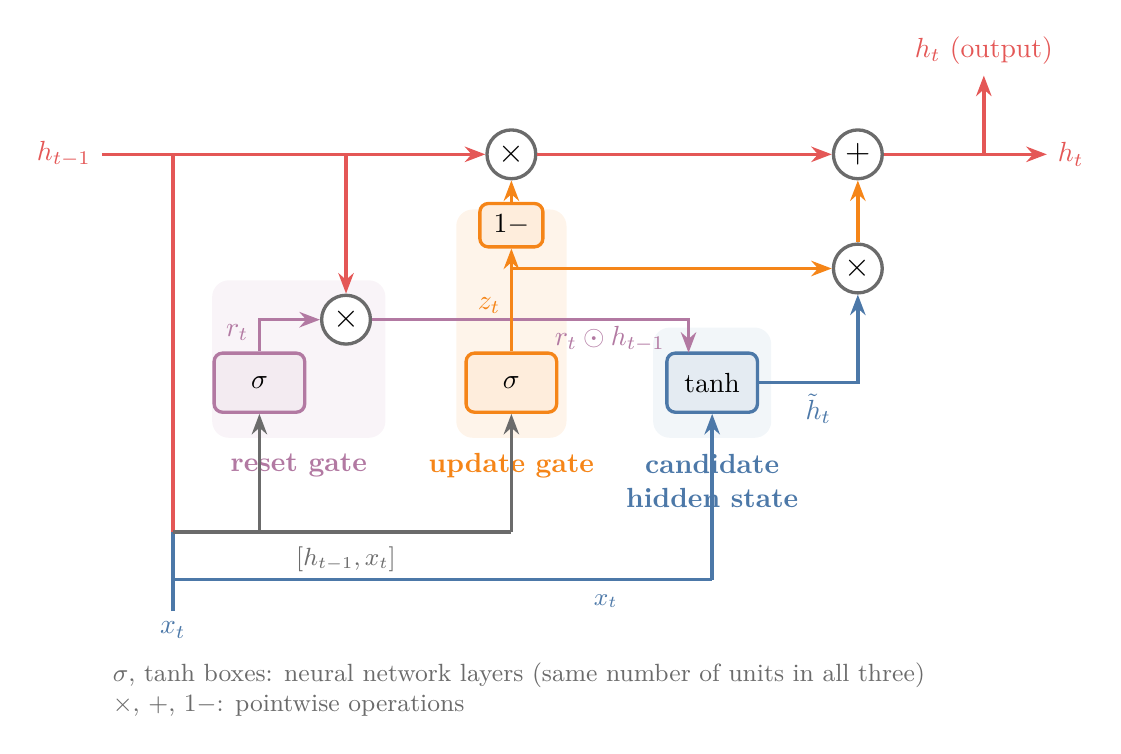
\begin{tikzpicture}[
  layer/.style={draw=#1, fill=#1!15, rounded corners=3pt, minimum width=1.15cm, minimum height=0.75cm, font=\sffamily},
  op/.style={circle, draw=cgrey, fill=white, minimum size=0.62cm, inner sep=0pt, font=\sffamily\large},
  line/.style={-{Stealth[length=2.6mm]}, line width=1.3pt}]
  % regions
  \fill[cpurple!8, rounded corners=6pt] (0.8,0.6) rectangle (3.0,2.6);
  \fill[corange!9, rounded corners=6pt] (3.9,0.6) rectangle (5.3,3.5);
  \fill[cblue!7, rounded corners=6pt] (6.4,0.6) rectangle (7.9,2.0);
  \node[font=\sffamily\bfseries, text=cpurple] at (1.9,0.25) {reset gate};
  \node[font=\sffamily\bfseries, text=corange] at (4.6,0.25) {update gate};
  \node[font=\sffamily\bfseries, text=cblue, align=center] at (7.15,0.05) {candidate\\hidden state};
  % top line: the hidden state
  \node[op] (keep) at (4.6,4.2) {$\times$};
  \node[op] (plus) at (9.0,4.2) {$+$};
  \draw[line, draw=cred] (-0.6,4.2) node[left, text=cred] {$h_{t-1}$} -- (keep);
  \draw[line, draw=cred] (keep) -- (plus);
  \draw[line, draw=cred] (plus) -- (11.4,4.2) node[right, text=cred] {$h_t$};
  \draw[line, draw=cred] (10.6,4.2) -- (10.6,5.2) node[above, text=cred] {$h_t$ (output)};
  % input bus [h_{t-1}, x_t]
  \draw[line width=1.3pt, draw=cred] (0.3,4.2) -- (0.3,-0.6);
  \draw[line width=1.3pt, draw=cblue] (0.3,-1.6) node[below, text=cblue] {$x_t$} -- (0.3,-0.6);
  \draw[line width=1.3pt, draw=cgrey] (0.3,-0.6) -- (4.6,-0.6);
  \node[note, anchor=north] at (2.5,-0.65) {$[h_{t-1}, x_t]$};
  \node[layer=cpurple] (r) at (1.4,1.3) {$\sigma$};
  \node[layer=corange] (z) at (4.6,1.3) {$\sigma$};
  \draw[line, draw=cgrey] (1.4,-0.6) -- (r);
  \draw[line, draw=cgrey] (4.6,-0.6) -- (z);
  % reset: r_t * h_{t-1}
  \node[op] (rx) at (2.5,2.1) {$\times$};
  \draw[line, draw=cred] (2.5,4.2) -- (rx);
  \draw[line, draw=cpurple] (r) |- node[pos=0.3, left, text=cpurple] {$r_t$} (rx);
  % candidate: tanh([r*h, x])
  \node[layer=cblue] (c) at (7.15,1.3) {tanh};
  \draw[line, draw=cpurple] (rx) -| (6.85,1.68);
  \node[text=cpurple, font=\sffamily] at (5.85,1.85) {$r_t \odot h_{t-1}$};
  \draw[line width=1.3pt, draw=cblue] (0.3,-1.2) -- (7.15,-1.2);
  \draw[line, draw=cblue] (7.15,-1.2) -- (c);
  \node[note, text=cblue, anchor=north] at (5.8,-1.25) {$x_t$};
  % update: (1 - z) on the old state, z on the candidate
  \node[layer=corange, minimum width=0.8cm, minimum height=0.55cm] (om) at (4.6,3.3) {$1-$};
  \draw[line, draw=corange] (z) -- node[left, pos=0.55, text=corange] {$z_t$} (4.6,2.75) -- (om);
  \draw[line, draw=corange] (om) -- (keep);
  \node[op] (zx) at (9.0,2.75) {$\times$};
  \draw[line, draw=corange] (4.6,2.75) -- (zx);
  \draw[line, draw=cblue] (c) -| node[pos=0.3, below, text=cblue] {$\tilde{h}_t$} (zx);
  \draw[line, draw=corange] (zx) -- (plus);
  % legend
  \node[note, anchor=west, align=left] at (-0.6,-2.6) {$\sigma$, tanh boxes: neural network layers (same number of units in all three)\\$\times$, $+$, $1-$: pointwise operations};
\end{tikzpicture}
\end{document}
